\documentclass[12pt]{beamer}
\usetheme{Warsaw}
\usepackage[utf8]{inputenc}
\usepackage{amsmath}
\usepackage{amsfonts}
\usepackage{amssymb}
\usepackage{graphicx}
\usepackage[font=Times,timeinterval=1,timeduration=2.0,timedeath=0,fillcolorwarningsecond=white!60!yellow,timewarningfirst=50,timewarningsecond=80,resetatpages=2]{tdclock}
\usepackage{tabularx}
\usepackage{array}
\usepackage{multicol}
\usepackage{longtable}
\usepackage{xcolor}
\usepackage{gensymb}
\usepackage{pgfplots}
\usepackage[makeroom]{cancel}

\graphicspath{ {./references/} }
\pgfplotsset{
	soldot/.style={color=black,only marks,mark=*},
	holdot/.style={color=black,fill=white,only marks,mark=*},
	compat=1.12
}
\newcolumntype{Y}{>{\centering\arraybackslash}X}
\makeatletter
\def\@listii{\leftmargin\leftmarginii
			  \topsep    2ex
			  \parsep    0\p@   \@plus\p@
			  \itemsep   \parsep}
\makeatother

\begin{document}
\begin{frame}
	\frametitle{Bellwork 10/2}
	\initclock

	\begin{center}
		\vfill
		Function $f$ is graphed below:
		\vfill
		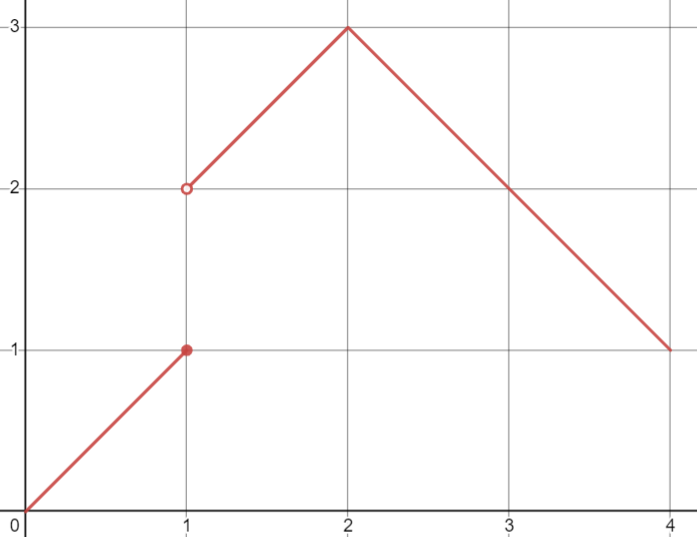
\includegraphics[scale=0.5]{bellwork_graph.png}
		\vfill
		Sketch $f'(x)$ and find where $f$ is not differentiable.
		\vfill
	\end{center}

	\small
	\crono
	\resetcrono{\beamerbutton{reset}}
\end{frame}
\begin{frame}
	\frametitle{Bellwork 10/2 - Solution}

	\begin{center}
		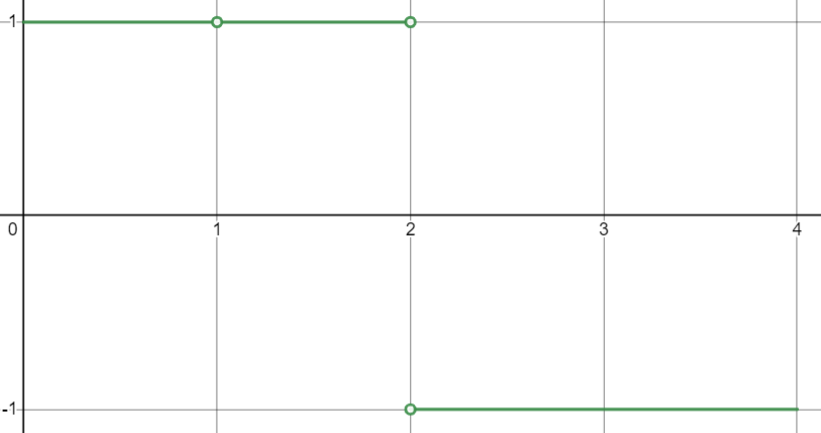
\includegraphics[scale=0.6]{bellwork_solution_graph.png}
		\vfill
		$\boxed{x=1\text{, }2}$
	\end{center}
\end{frame}
\begin{frame}
	\frametitle{Exercise 1}
	
	\begin{center}
		\vfill
		Function $f$ is graphed below:
		\vfill
		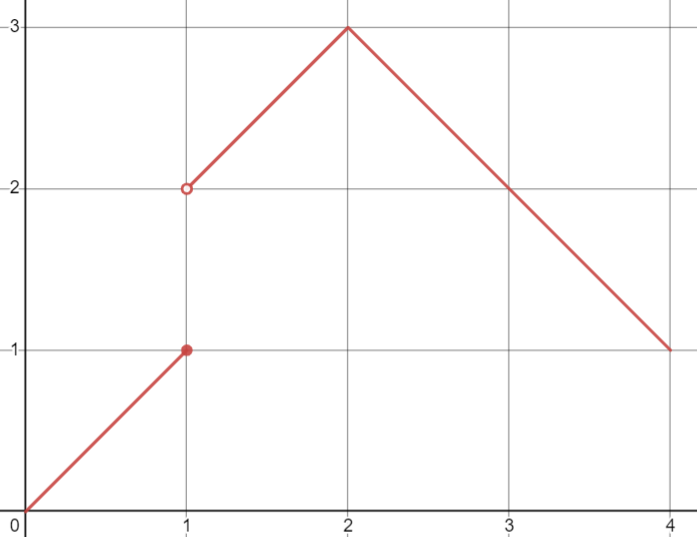
\includegraphics[scale=0.5]{exercise_1_graph.png}
		\vfill
		Sketch $f'(x)$ and find where $f$ is not differentiable.
		\vfill
	\end{center}
\end{frame}
\begin{frame}
	\frametitle{Exercise 1 - Solution}

	\begin{center}
		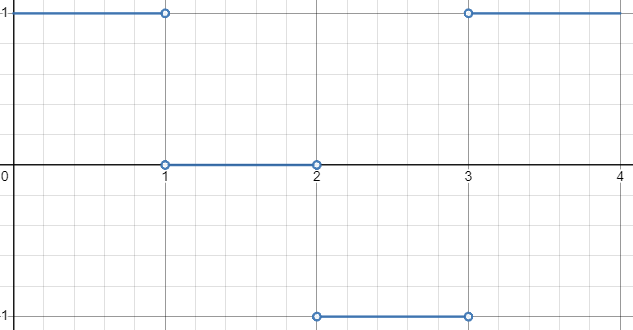
\includegraphics[scale=0.6]{exercise_1_solution_graph.png}
		\vfill
		$\boxed{x=1\text{, }2\text{, }3}$
	\end{center}
\end{frame}
\end{document}